\documentclass[11pt,twocolumn,twoside]{opticajnl}
%% Please use 11pt if submitting to AOP
% \documentclass[11pt,twocolumn,twoside]{opticajnl}

\journal{pr} % Choose journal (ao,jocn,josaa,josab,ol,optica,pr)

%See template introduciton for guidance on setting shortarticle option
\setboolean{shortarticle}{True}
% true = letter/tutorial
% false = research/review article
% (depending on journal)
\usepackage{lineno}
\usepackage[utf8]{inputenc}
\spanishdecimal{.}
\usepackage{amsmath}
\usepackage{caption}
\usepackage{subcaption}
\usepackage[spanish]{babel}
\usepackage{hyperref}
\usepackage{listings}
\usepackage{multicol}
%\linenumbers
\lstdefinestyle{mystyle}{
    language=Python, % Choose the programming language (e.g., Python)
    basicstyle=\ttfamily, % Set the font style
    keywordstyle=\color{blue}, % Define the color for keywords
    commentstyle=\color{green!40!black}, % Define the color for comments
    numbers=left, % Show line numbers
    numberstyle=\tiny, % Set the style for line numbers
    frame=single, % Add a frame around the code
    breaklines=true, % Allow line breaks within code
    showstringspaces=false % Don't show spaces within strings
}


% Configura el formato del título del listado
\renewcommand\lstlistingname{Código}
\renewcommand\lstlistlistingname{Códigos}
\title{
\vspace{0.1cm} 

Trabajo práctico 4: Aprendizaje no supervisado}

\author[1]{\huge{Ignacio Lembo Ferrari}}
\affil[1]{\large{ignaciolembo@ib.edu.ar} 

\vspace{0.1cm}

{\datesfont 31 de octubre del 2023.}

\vspace{0.1cm}
}

%\begin{abstract}
%\textbf{hola}
%\end{abstract}

\begin{document}

\maketitle

\section{Red de una capa lineal: Implementación de la regla de Oja \label{sec:ej1}}

\vspace{0.3cm}

Se utilizó una red de una capa lineal con 4 entradas y una salida. La ecuación de salida es
\begin{equation}
    V = \sum_{j=1}^{4} w_j \xi_j.
\end{equation}
La distribución de probabilidad de las entradas es una distribución gaussiana
\begin{equation}
    P(\vec{\zeta}) = \frac{1}{(2\pi)^2 \sqrt{\Sigma}} \exp(-\frac{1}{2} \vec{\zeta}^T \Sigma^{-1} \vec{\zeta})
    \label{eq:dist_gauss}
\end{equation}
donde $\Sigma$ es la matriz de correlación 
\begin{equation}
    \Sigma = \begin{pmatrix}
        2 & 1 & 1 & 1 \\ 
        1 & 2 & 1 & 1 \\
        1 & 1 & 2 & 1 \\
        1 & 1 & 1 & 2
    \end{pmatrix}
\end{equation}

Partiendo de pesos iniciales pequeños dados por una distribución uniforme en el intervalo $[-0.1,0.1]$, se entrenó una red con datos de entrada $\xi$ generados de la siguiente manera: En cada época, se generaron vectores $\zeta$ cuyas componentes se calcularon a partir de distribuciones de probabilidad gaussianas independientes dada por la Ec. \ref{eq:dist_gauss}. Luego, los vectores $\xi$ se calcularon como
\begin{equation}
    \xi = \Sigma^{1/2} \zeta,
\end{equation}  
de modo tal que estos nuevos vectores no tienen correlación entre sus componentes. Para actualizar los pesos en cada época, se utilizó la regla de Oja dada por 
\begin{equation}
    \Delta w_{j} = \eta V (\xi_j - V~w_j).
\end{equation}
donde $\eta$ es la tasa de aprendizaje.

En el aprendizaje dado por la regla de Oja el vector de pesos se alinea con el autovector correspondiente al máximo autovalor de la matriz de correlación $\Sigma$. En este caso los autovalores de la matriz $\Sigma$ son $\lambda = 1$ con multiplicidad 3 y $\lambda = 5$. En particular el autovector correspondiente al máximo autovalor $\lambda = 5$ es $\vec{v_1} = (0.5,0.5,0.5,0.5)$. Vale destacar que el vector de pesos también se podría alinear con vector antiparalelo a $\vec{v_1}$, osea $-\vec{v_1} = (-0.5,-0.5,-0.5,-0.5)$. Se realizaron estudios para distintas tasas de aprendizaje. En la Fig. \ref{fig:pesos_epocas} se muestra la evolución de las componentes del vector de pesos $\vec{w} = (w_1,w_2,w_3,w_4)$ en función de las épocas. Se observa que las componentes de dicho vector convergen a las componentes del autovector $\vec{v_1}$ o $-\vec{v_1}$. 

\begin{figure}[h]
    \centering
         \begin{subfigure}[b]{0.49\linewidth}
            \centering
            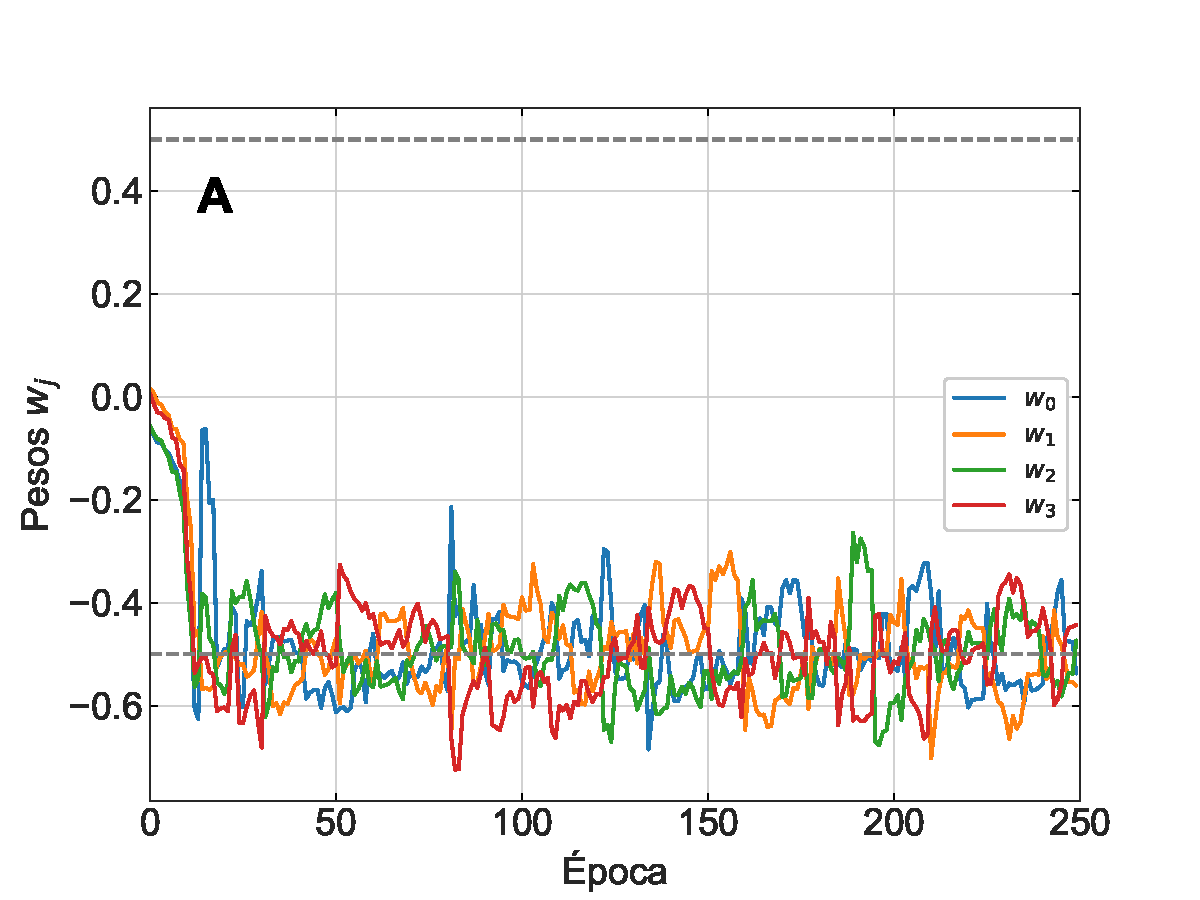
\includegraphics[width=1.1\textwidth]{Figuras/pesos_lr_0.01.pdf}
         \end{subfigure}
         \begin{subfigure}[b]{0.49\linewidth}
            \centering
            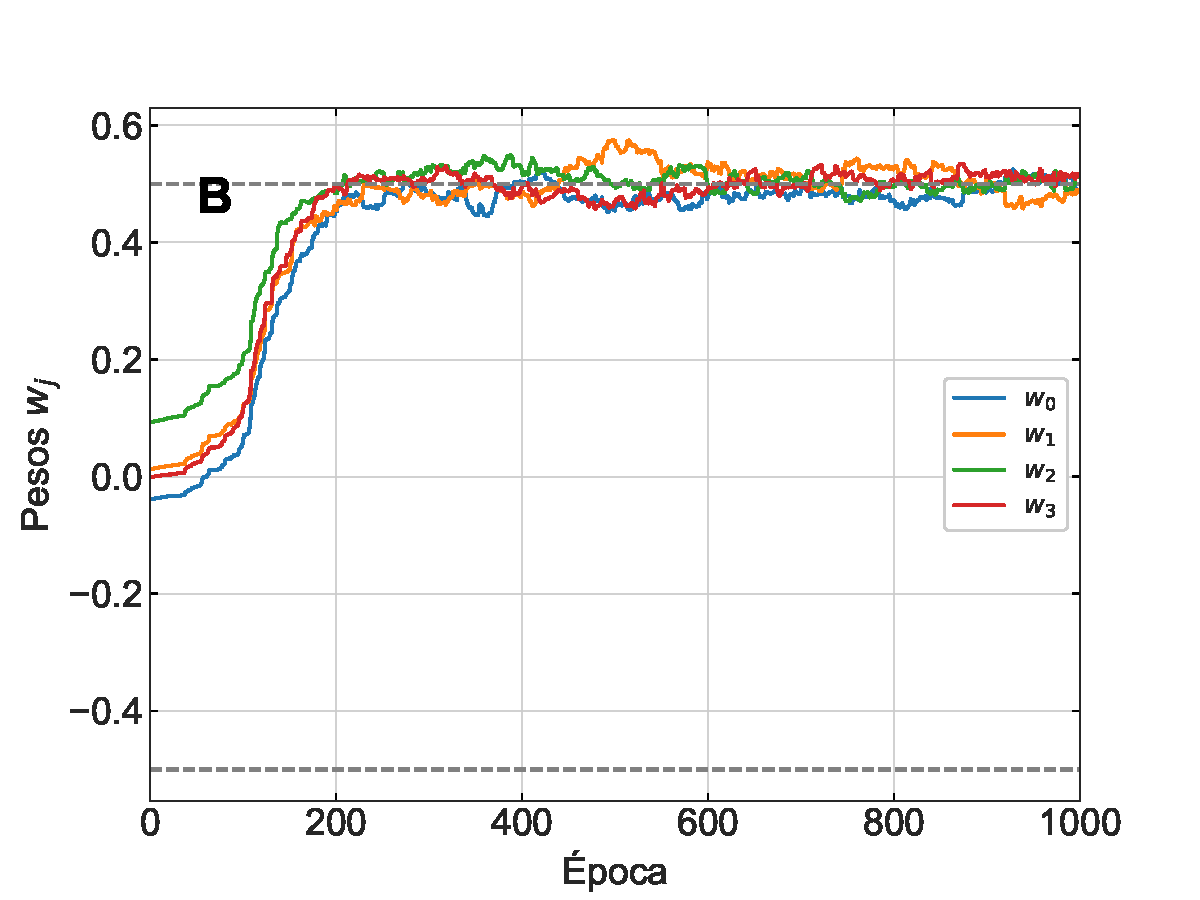
\includegraphics[width=1.1\textwidth]{Figuras/pesos_lr_0.001.pdf}
         \end{subfigure}
         \begin{subfigure}[b]{0.49\linewidth}
            \centering
            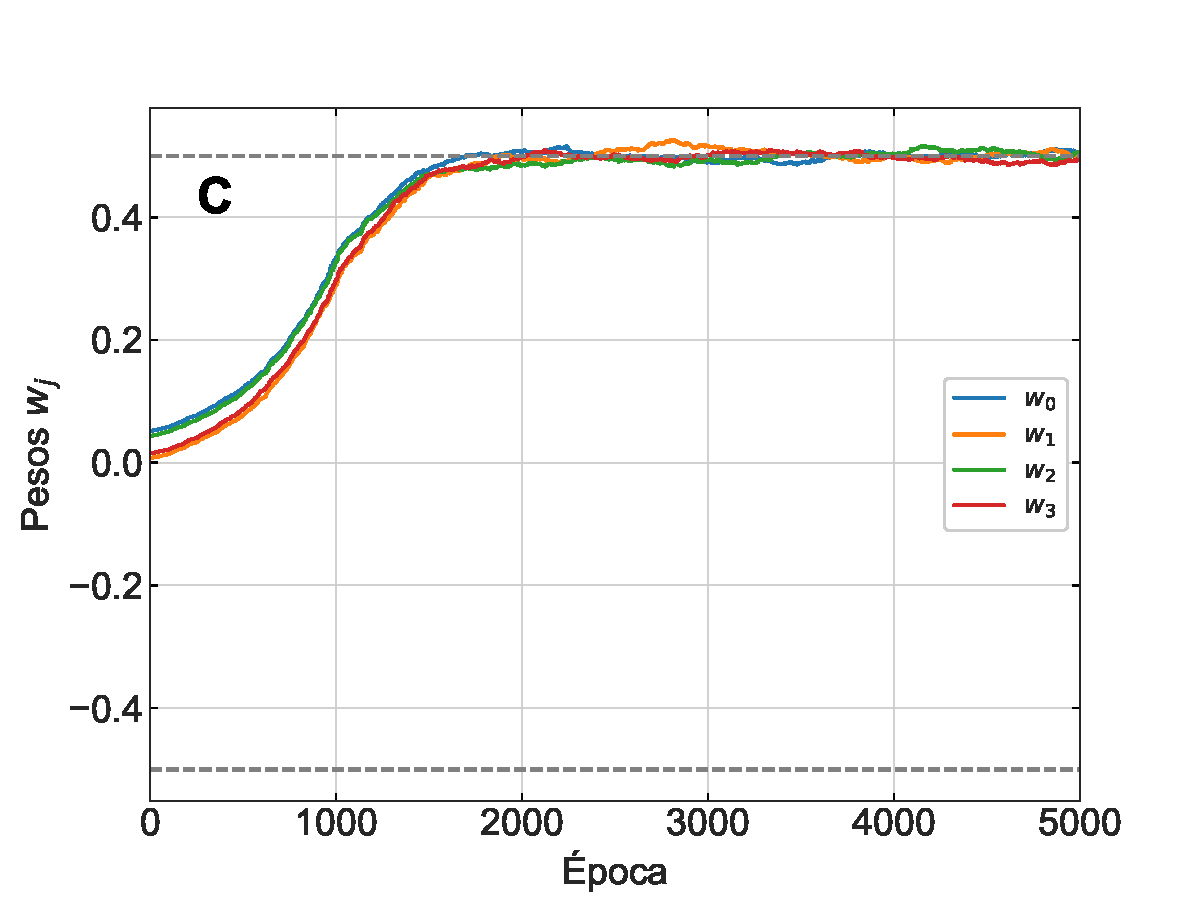
\includegraphics[width=1.1\textwidth]{Figuras/pesos_lr_0.0001.pdf}
         \end{subfigure}
         \begin{subfigure}[b]{0.49\linewidth}
            \centering
            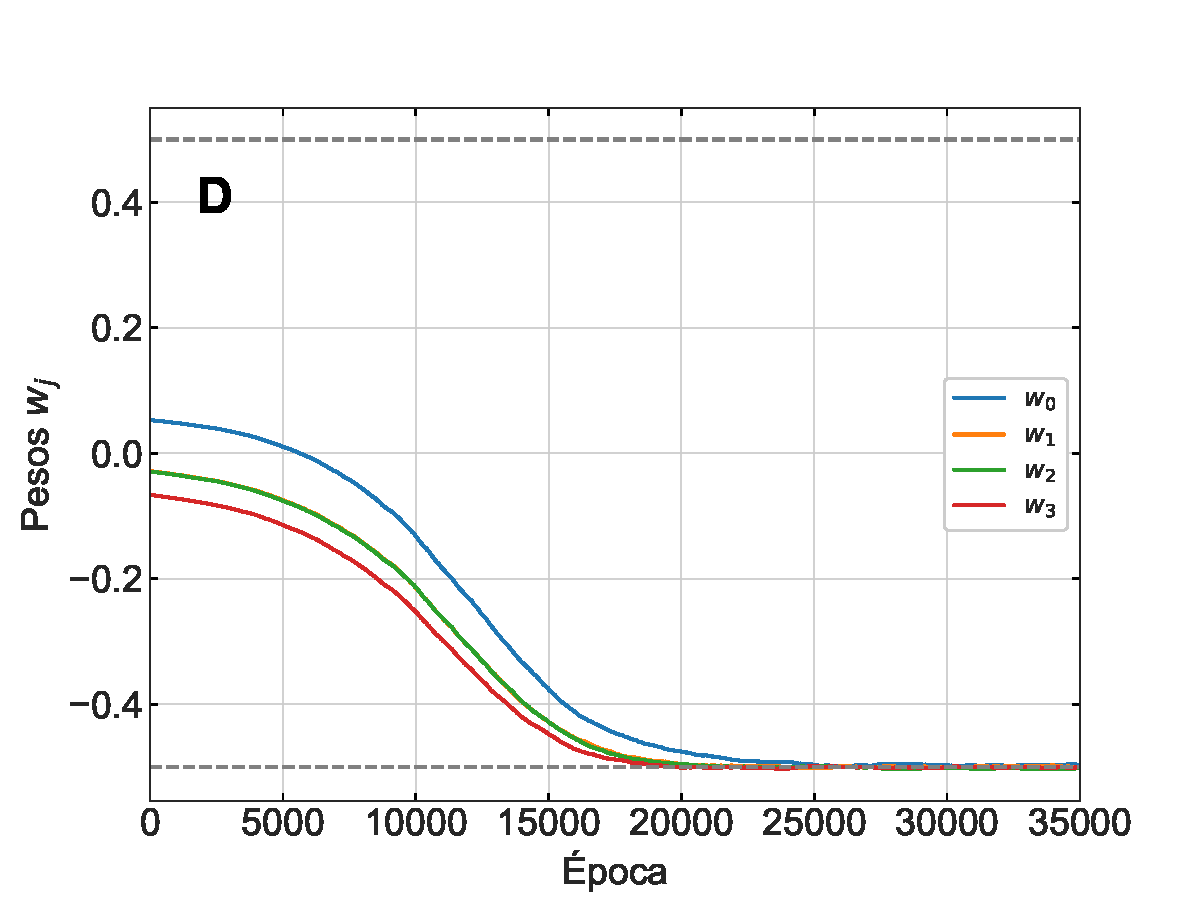
\includegraphics[width=1.1\textwidth]{Figuras/pesos_lr_1e-05.pdf}
         \end{subfigure}
    \caption{Evolución de los pesos de la red neuronal para (A) $\eta=0.01$, (B) $\eta=0.001$, (C) $\eta=0.0001$ y (D) $\eta=0.00001$} 
    \label{fig:pesos_epocas}
\end{figure}

En la Fig. \ref{fig:prodesc_epocas} se muestra la evolución del producto escalar del vector de pesos con los autovectores de la matriz $\Sigma$ en función de las épocas. Se observa que el producto escalar con el autovector $\vec{v_1}$ correspondiente al máximo autovalor de $\Sigma$ converge a $1$ o $-1$ mientras que los productos escalares con el resto de los autovectores corresponde a 0, indicando que $\vec{w}$ es ortogonal a los mismos.

En todos los casos se observa que al aumentar la tasa de aprendizaje las curvas son menos ruidosas pero a la red neuronal le lleva más épocas converger a los valores mencionados. No obstante, siempre converge a los valores mencionados para todas las tasas de aprendizaje.

\begin{figure}[h]
    \centering
         \begin{subfigure}[b]{0.49\linewidth}
            \centering
            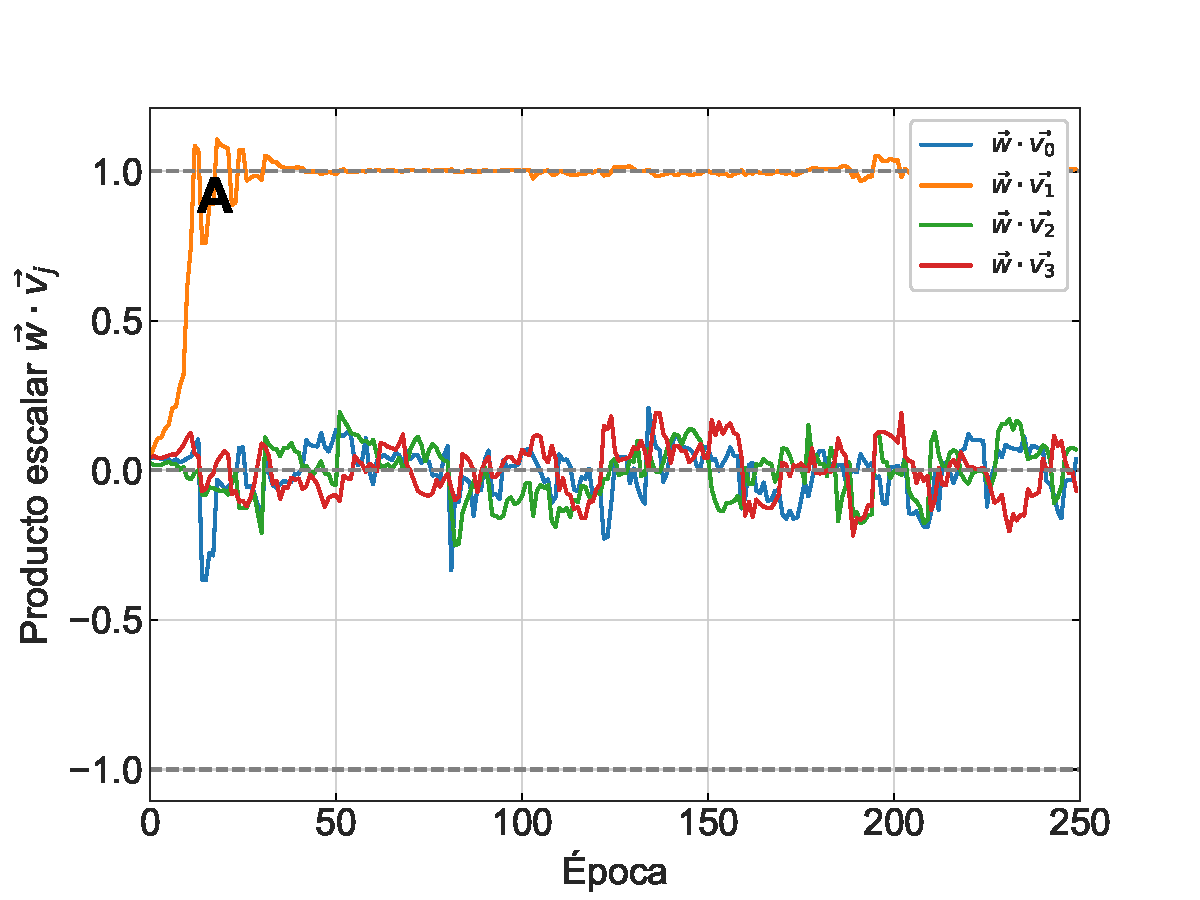
\includegraphics[width=1.1\textwidth]{Figuras/prodesc_lr_0.01.pdf}
         \end{subfigure}
         \begin{subfigure}[b]{0.49\linewidth}
            \centering
            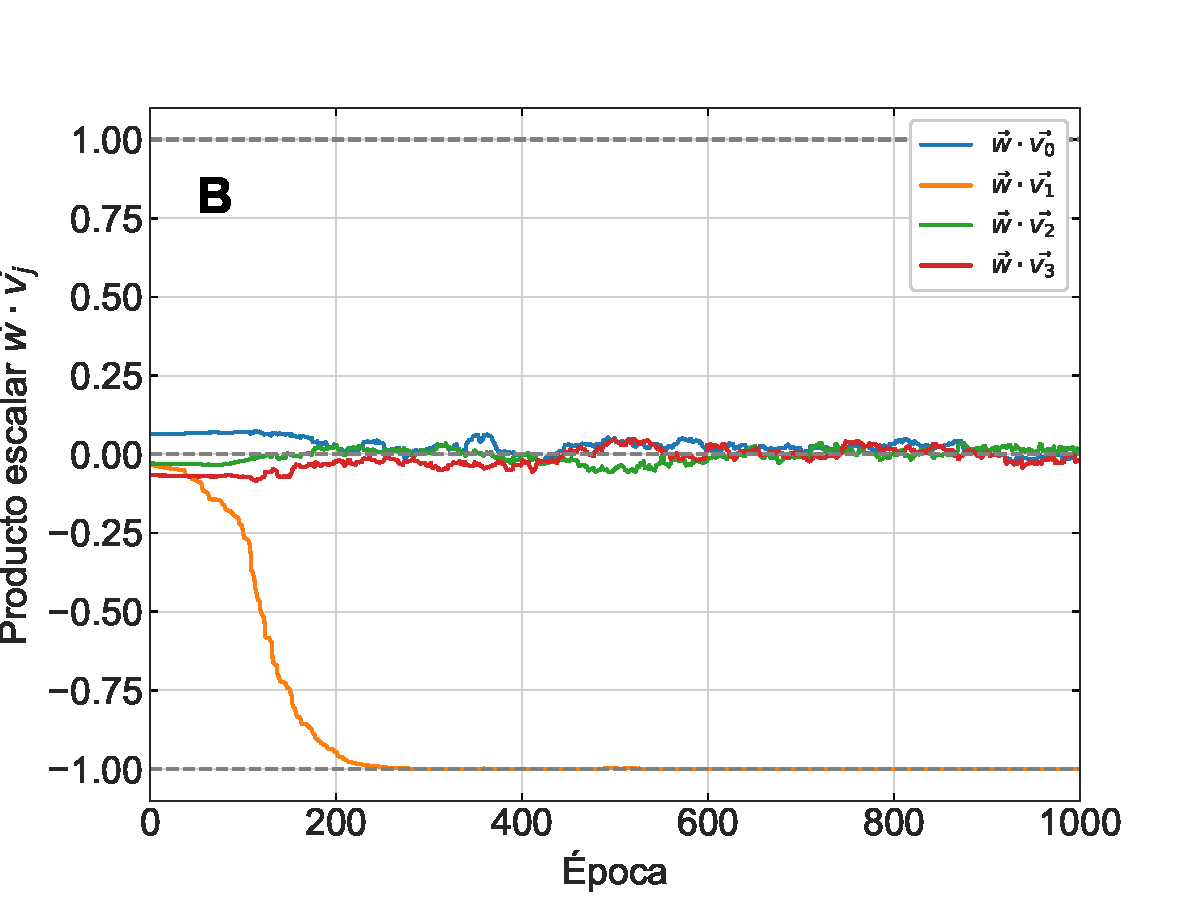
\includegraphics[width=1.1\textwidth]{Figuras/prodesc_lr_0.001.pdf}
         \end{subfigure}
         \begin{subfigure}[b]{0.49\linewidth}
            \centering
            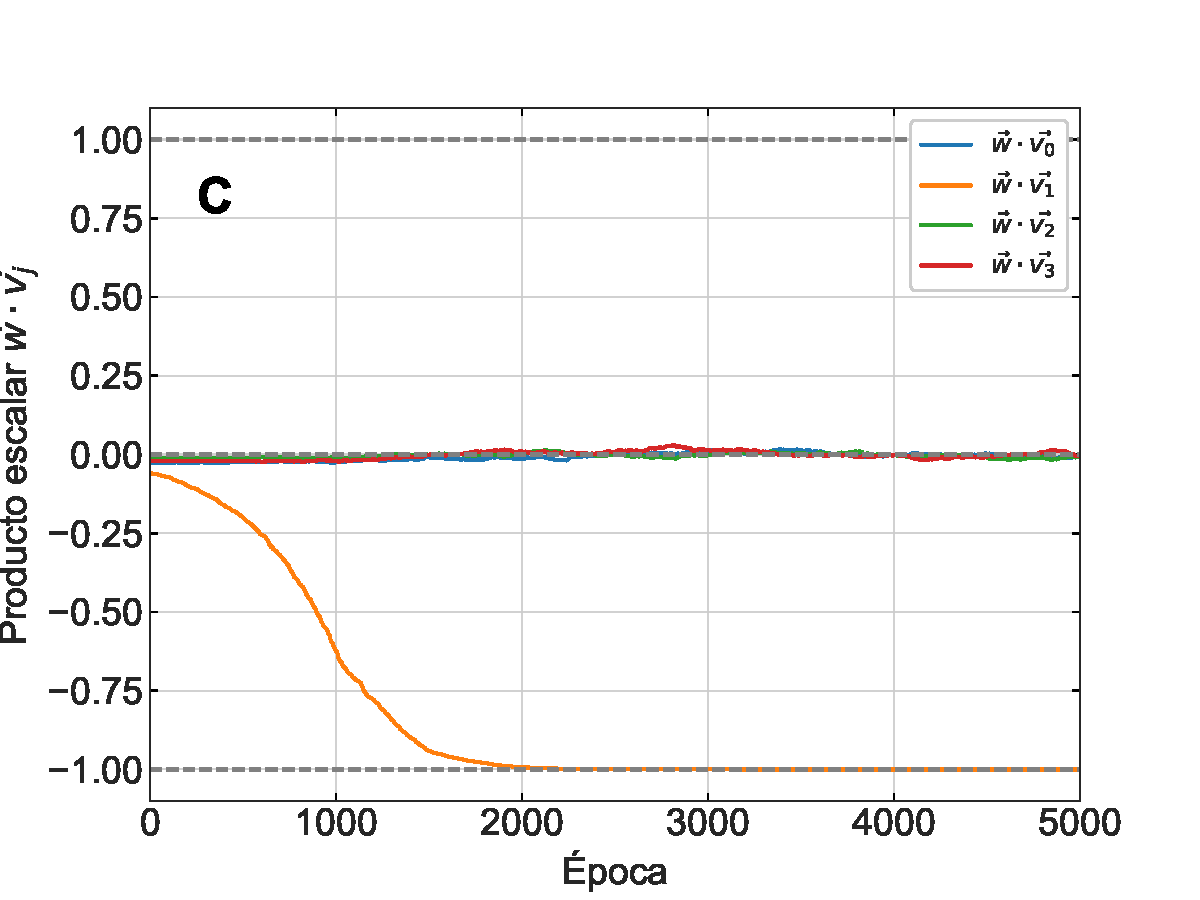
\includegraphics[width=1.1\textwidth]{Figuras/prodesc_lr_0.0001.pdf}
         \end{subfigure}
         \begin{subfigure}[b]{0.49\linewidth}
            \centering
            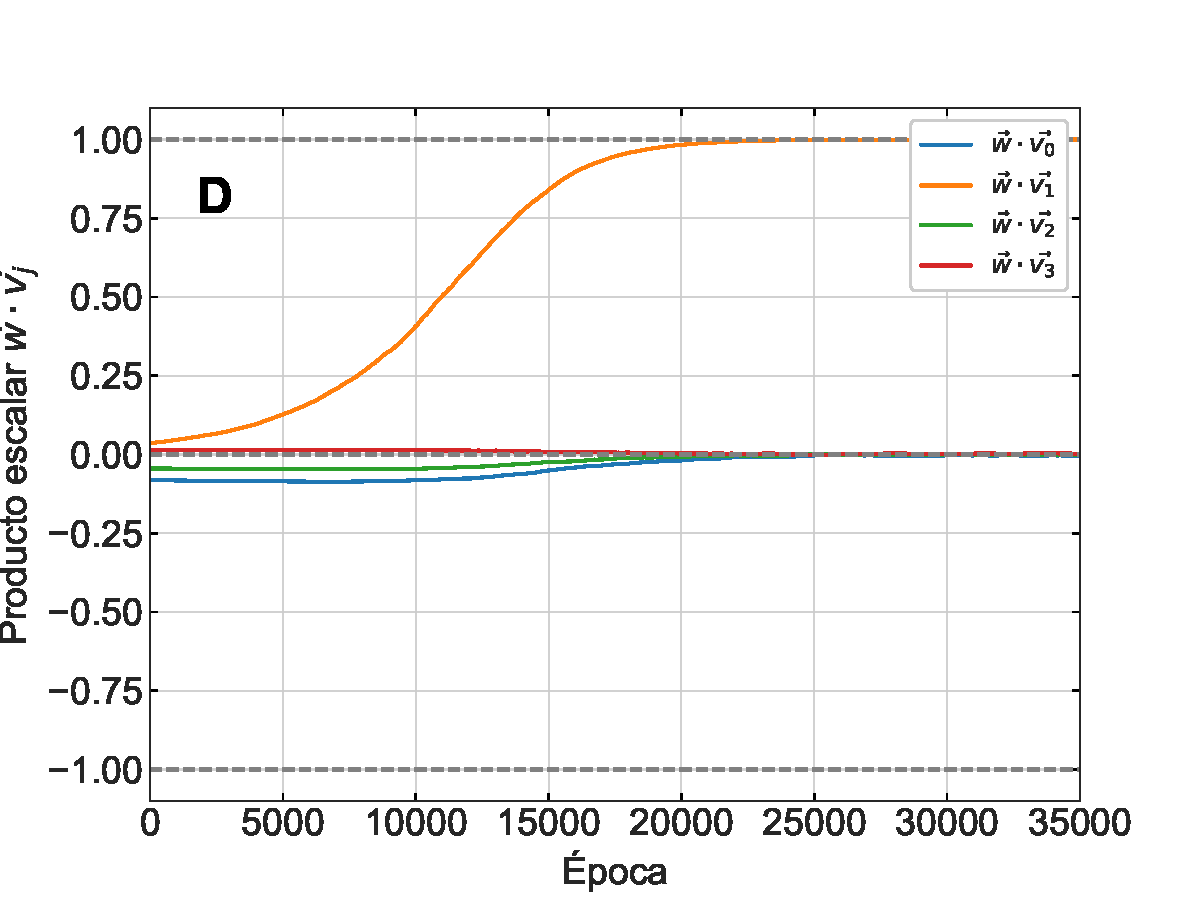
\includegraphics[width=1.1\textwidth]{Figuras/prodesc_lr_1e-05.pdf}
         \end{subfigure}
    \caption{Evolución del producto escalar del vector pesos con los autovectores de la matriz $\Sigma$ para (A) $\eta=0.01$, (B) $\eta=0.001$, (C) $\eta=0.0001$ y (D) $\eta=0.00001$. El autovector $\vec{v_1}$ corresponde al máximo autovalor $\lambda = 5$ de la matriz $\Sigma$.} 
    \label{fig:prodesc_epocas}
\end{figure}


\section{Red neuronal de Kohonen \label{sec:ej1}}

\vspace{0.3cm}

La red neuronal de Kohonen es una red neuronal artificial no supervisada que se utiliza para el aprendizaje competitivo de mapas topológicos. Se implementó dicha red con dos neuronas de entrada y diez neuronas de salida. 

En cada paso de aprendizaje se selecciona una neurona de salida $i^*$ que minimiza la distancia euclídea $||\vec{\xi} - \vec{w_i}||$. Luego, se actualizan los pesos de la neurona seleccionada y de sus vecinas de acuerdo a la regla de aprendizaje de Kohonen dada por
\begin{equation}
    \Delta w_{ij} = \eta \Lambda(i,i^*) (\xi_i - w_{ij})
\end{equation}
donde $\eta$ es la tasa de aprendizaje y $\Lambda$ es la función vecindad. En este trabajo se utilizó la función vecindad gaussiana dada por 
\begin{equation}
    \Lambda \propto \exp(-\frac{(i-i^*)^2}{2\sigma^2}).
\end{equation}
La función vecindad se utiliza para determinar el grado de influencia de las neuronas vecinas en la actualización de los pesos de la neurona seleccionada. Es decir, para valores grandes de $\sigma$ la función vecindad es más ancha, por lo que las neuronas de salida se ven más afectadas por las neuronas vecinas. En cambio, para valores pequeños de $\sigma$ la actualización de los pesos es más local y las neuronas no se afectan tanto entre sí. 

\subsection{Evolución temporal de la red}

Para estudiar el efecto del tiempo de entrenamiento en la posición asintótica de los pesos sinápticos, se iniciaron los pesos de cada neurona de salida en coordenas aleatorias en el rango $x \in [-0.2,0.2]$ e $y \in [0,0.2]$. Se alimentó las neuronas de entrada con una distribución 
\begin{equation}
    P(\vec{\xi}) = P(r,\theta) = 
    \begin{cases}
        \text{constante si } r \in [0.9,1.1],~ \theta \in [0,\pi] \\
        0 \text{ si no}
    \end{cases}
\end{equation}
donde $r$ y $\theta$ son las coordenadas polares del vector $\xi$. Se utilizó la función vecindad gaussiana 

En la Fig. \ref{fig:Kohonen_epocas} se muestra la trayectoria de las neuronas de salida para distintas épocas. Se observa que, al evolucionar la red temporalmente, las neuronas convergen rápidamente en dirección radial hacia el anillo, pero luego se observa una evolución muy lenta en dirección tangencial. Luego de las 100000 épocas se observan cambios muy pequeños. Se puede ver, para valores grandes de épocas, como las neuronas se ordenan en el anillo cubriendo todo el espacio.

\begin{figure*}[h]
    \centering
         \begin{subfigure}[b]{0.33\linewidth}
            \centering
            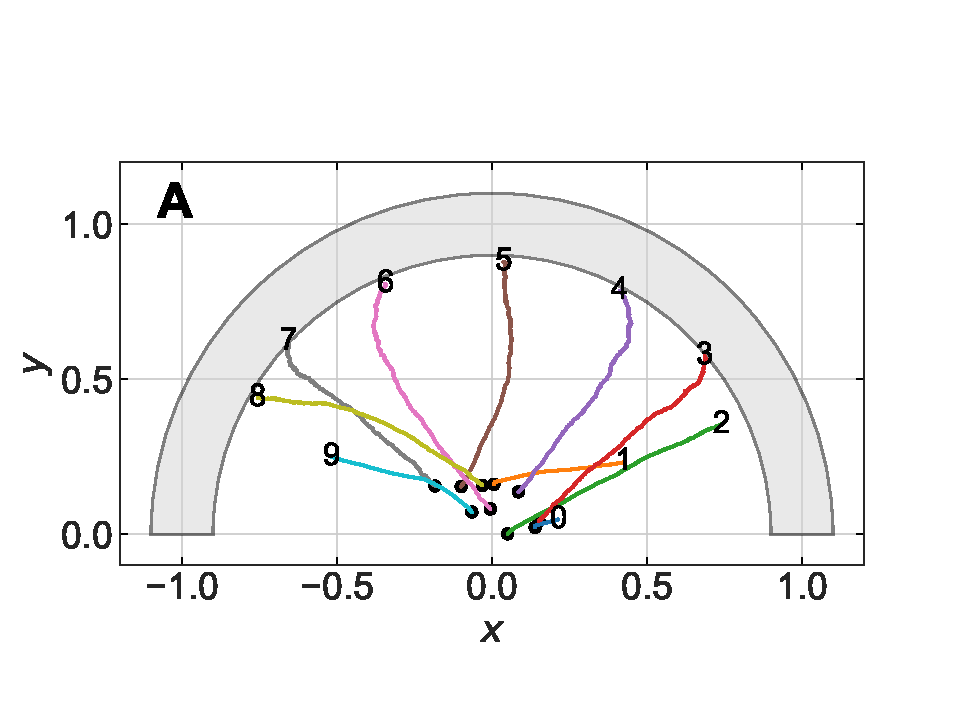
\includegraphics[width=1.1\textwidth]{Figuras/pesos_sigma_1_epochs_10000_lr_0.001.pdf}
         \end{subfigure}
         \begin{subfigure}[b]{0.33\linewidth}
            \centering
            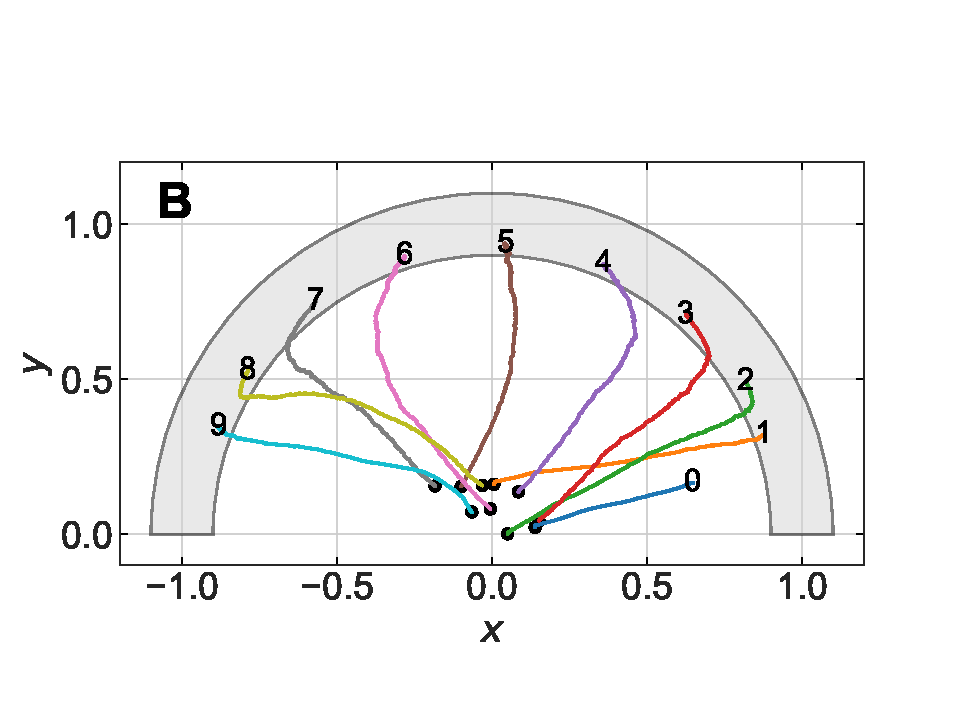
\includegraphics[width=1.1\textwidth]{Figuras/pesos_sigma_1_epochs_25000_lr_0.001.pdf}
         \end{subfigure}
         \begin{subfigure}[b]{0.33\linewidth}
            \centering
            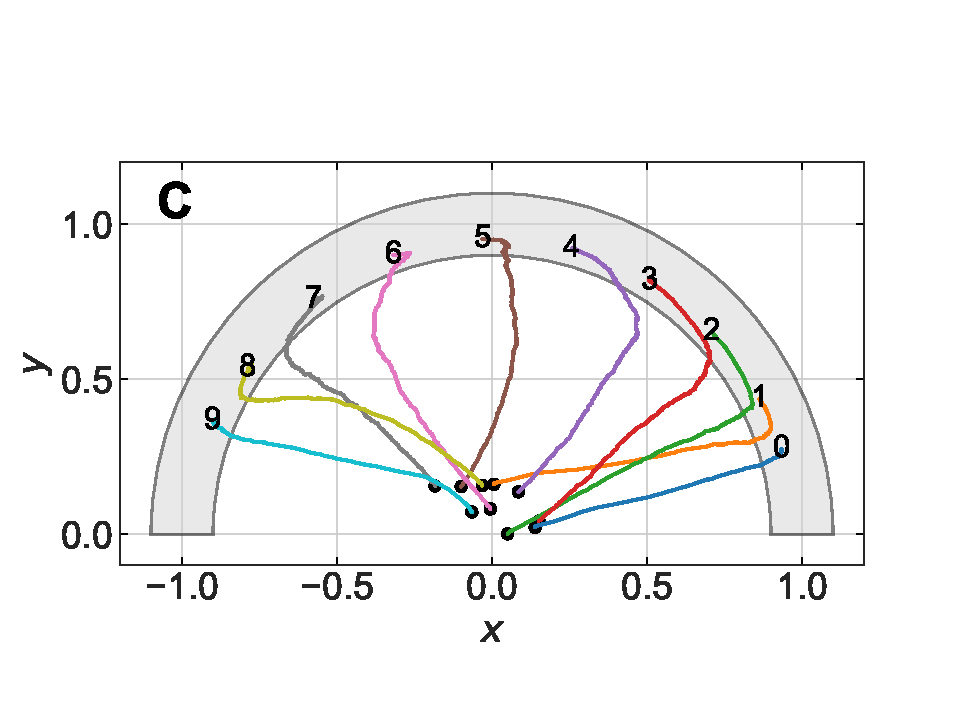
\includegraphics[width=1.1\textwidth]{Figuras/pesos_sigma_1_epochs_50000_lr_0.001.pdf}
         \end{subfigure}
         \begin{subfigure}[b]{0.33\linewidth}
            \centering
            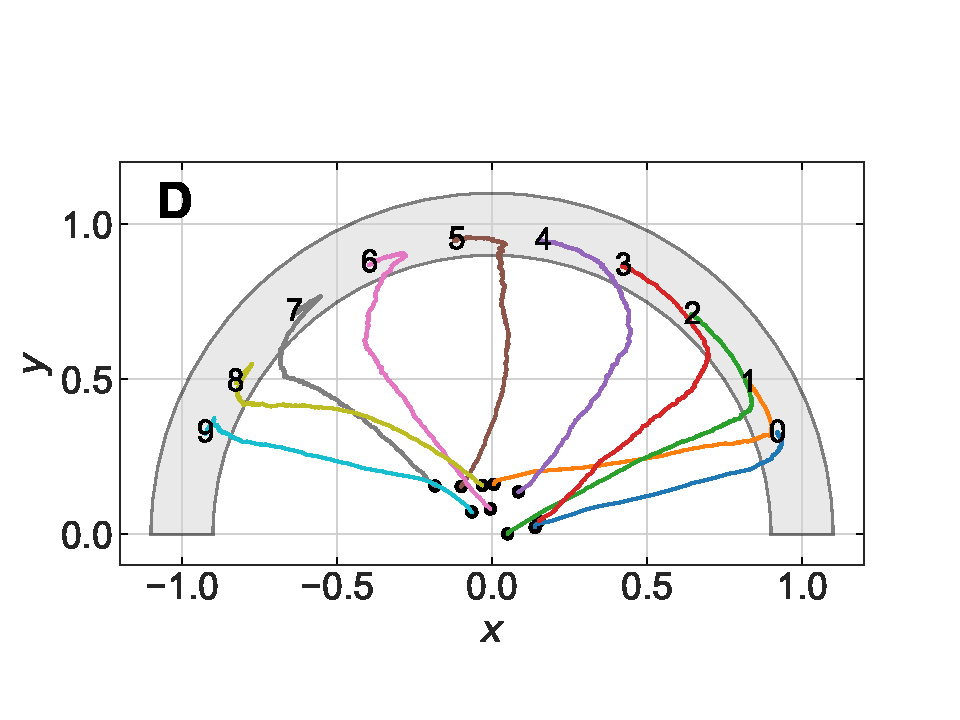
\includegraphics[width=1.1\textwidth]{Figuras/pesos_sigma_1.0_epochs_100000_lr_0.001_ev.pdf}
         \end{subfigure}
         \begin{subfigure}[b]{0.33\linewidth}
            \centering
            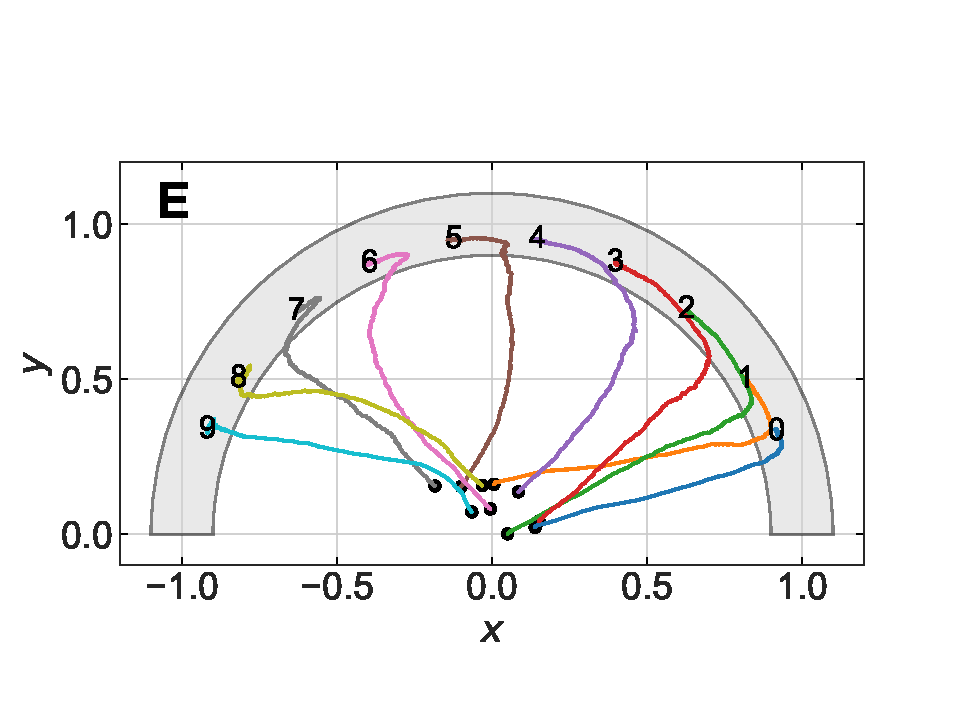
\includegraphics[width=1.1\textwidth]{Figuras/pesos_sigma_1_epochs_200000_lr_0.001.pdf}
         \end{subfigure}
         \begin{subfigure}[b]{0.33\linewidth}
            \centering
            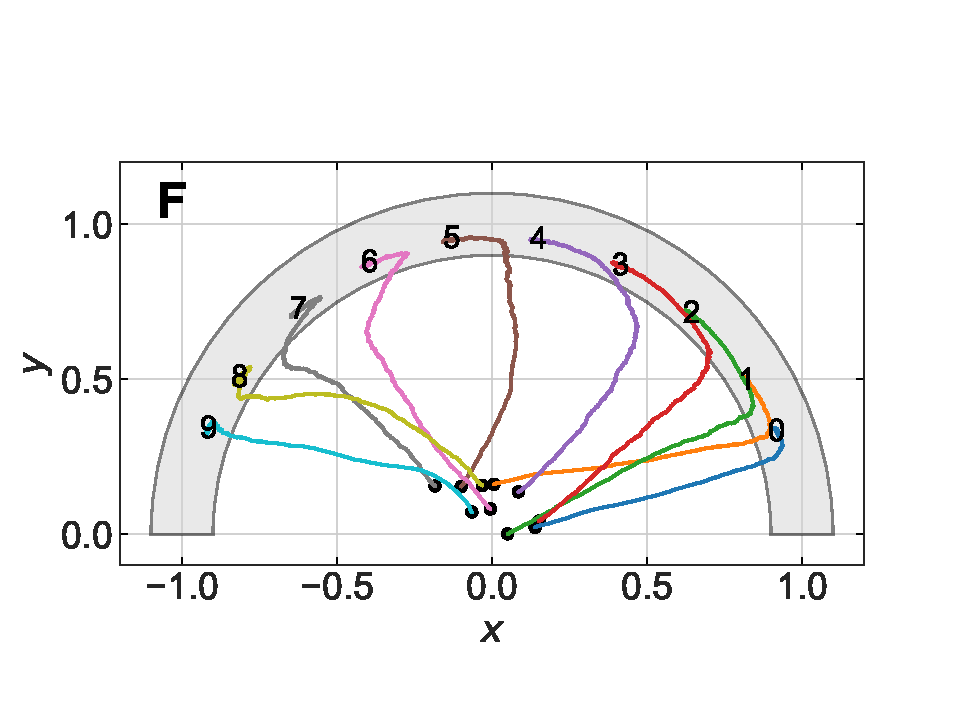
\includegraphics[width=1.1\textwidth]{Figuras/pesos_sigma_1_epochs_500000_lr_0.001.pdf}
         \end{subfigure}
    \caption{Trayectoria de las neuronas de salida para una red de Kohonen con $\sigma=1$, $\eta=0.001$ y (A) 10000 épocas, (B) 25000 épocas, (C) 50000 épocas y (D) 100000 épocas, (E) 200000 épocas, (F) 500000 épocas.} 
    \label{fig:Kohonen_epocas}
\end{figure*}

\subsection{Efecto del parámetro $\sigma$ en la evolución de la red \label{sec:sigma}}

Se realizaron experimentos para distintos valores del parámetro $\sigma$ de la función vecindad gaussiana. En la Fig. \ref{fig:Kohonen_sigma} se muestra la trayectoria de las neuronas de salida entrenadas con $\eta=0.001$ y $100000$ épocas para distintos valores de $\sigma$. Se observa que para valores grandes de $\sigma$ la evolución de la red cubre más espacio y las neuronas se encuentran más superpuestas pero no se encuentran centradas en el anillo, si no, en el borde interior del mismo. Las neuronas siempre se ordenan. Para valores pequeños de $\sigma$, en particular para $\sigma=0.5$, si bien hay un orden, no es tan claro como en el resto de los casos y se observa que sólo algunas neuronas llegan a evolucionar hasta el anillo, esto se debe a que la función vecindad es muy angosta, por lo que las neuronas de salida se ven menos afectadas por las neuronas vecinas. Luego, hay neuronas, cuya actualización de pesos practicamente no se modifica al ser tan localizada la función $\Lambda$.

\begin{figure}[H]
    \centering
         \begin{subfigure}[b]{0.49\linewidth}
            \centering
            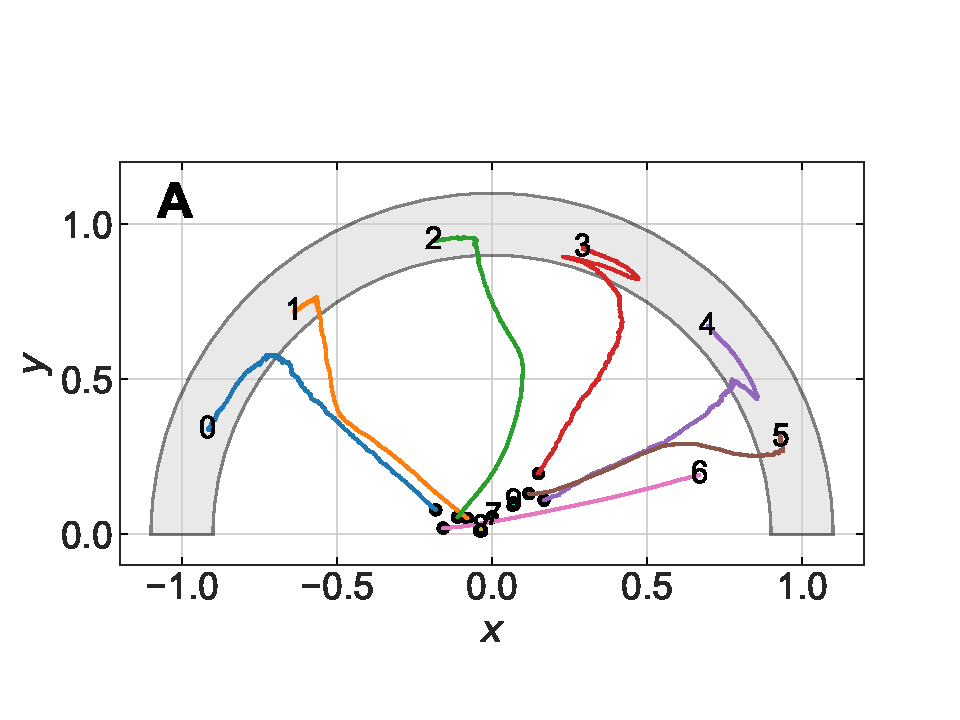
\includegraphics[width=1.1\textwidth]{Figuras/pesos_sigma_0.5_epochs_100000_lr_0.001.pdf}
         \end{subfigure}
         \begin{subfigure}[b]{0.49\linewidth}
            \centering
            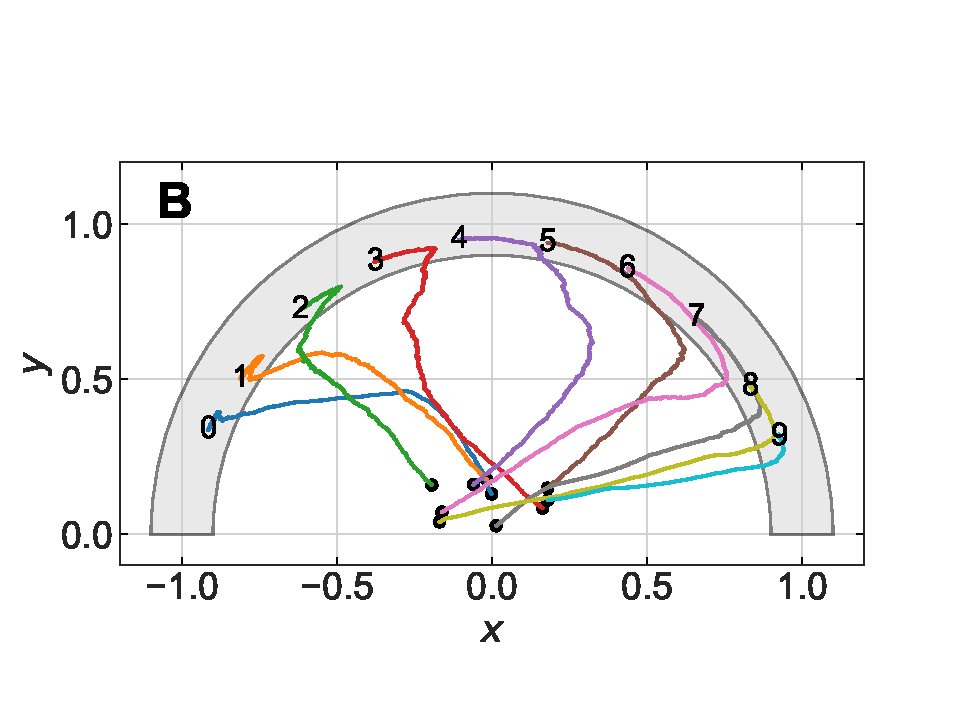
\includegraphics[width=1.1\textwidth]{Figuras/pesos_sigma_1_epochs_100000_lr_0.001.pdf}
         \end{subfigure}
         \begin{subfigure}[b]{0.49\linewidth}
            \centering
            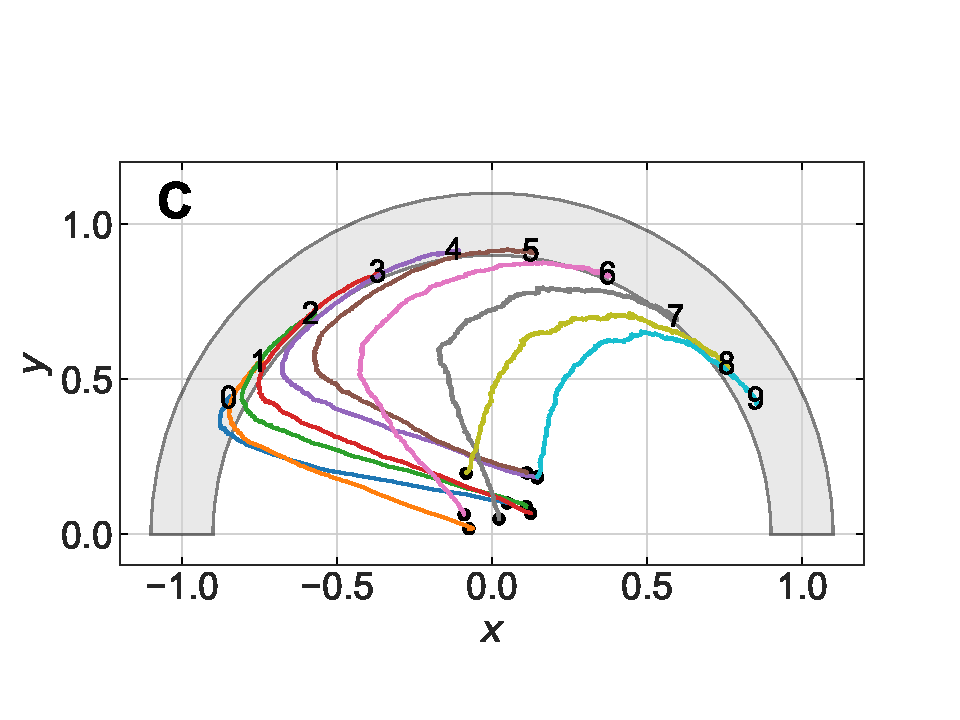
\includegraphics[width=1.1\textwidth]{Figuras/pesos_sigma_1.5_epochs_100000_lr_0.001.pdf}
         \end{subfigure}
         \begin{subfigure}[b]{0.49\linewidth}
            \centering
            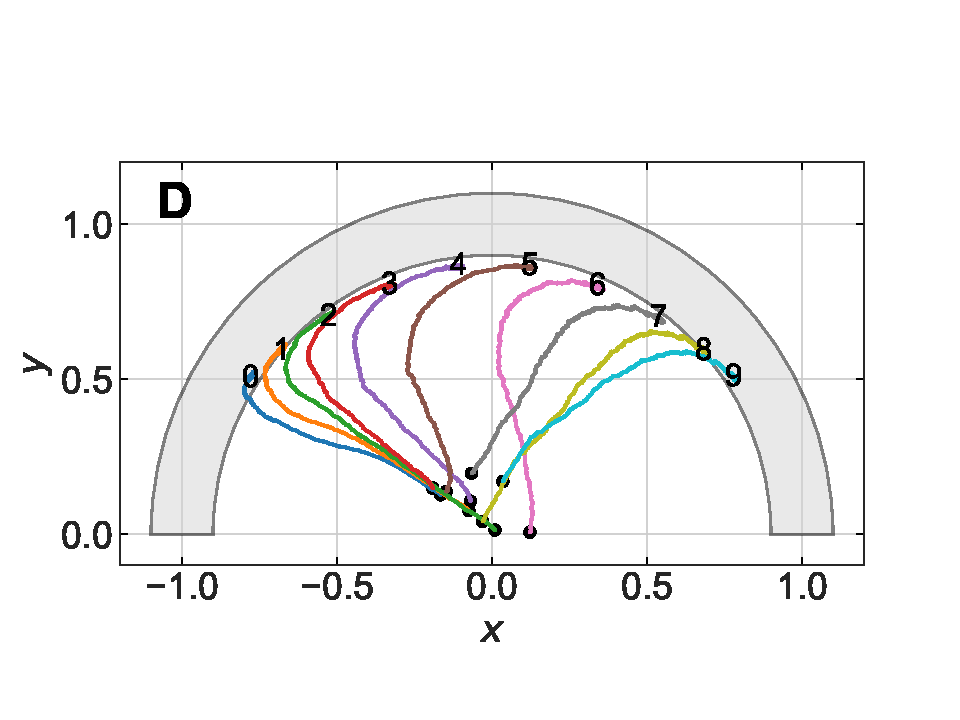
\includegraphics[width=1.1\textwidth]{Figuras/pesos_sigma_2_epochs_100000_lr_0.001.pdf}
         \end{subfigure}
    \caption{Trayectoria de las neuronas de salida para una red de Kohonen con $\eta=0.001$ para $100000$ épocas y (A) $\sigma=0.5$, (B) $\sigma=1.0$, (C) $\sigma=1.5$ y (D) $\sigma=2.0$.} 
    \label{fig:Kohonen_sigma}
\end{figure}


\subsection{Parámetro $\sigma$ adaptativo}

Insipirado en la sección anterior (\ref{sec:sigma}) se implementó un parámetro $\sigma$ adaptativo que disminuye con el tiempo de entrenamiento de la forma $\sigma(t) = \sigma_0/t$ y se realizaron experimentos similares a los de dicha sección. Se alimentó la red con entradas dadas por una distribución constante dentro de una semicorona, un triángulo equilátero y un cuadrado donde la probabilidad de tener una entrada en la mitad superior del mismo es el doble que en la mitad inferior. En todos los casos, se entrenó a la red durante $100000$ épocas y $\eta=0.01$. 

En el primer experimento, los pesos iniciales se tomaron en una región pequeña de modo que las neuronas empiezan todas cerca. En la Fig. \ref{fig:Kohonen_sigma_adp} se observa que las neuronas inicialmente se mueven todas juntas y luego en un punto se separan, cubriendo todo la topología de las neuronas de entrada. Se detectó que, este punto, para todas las topologías estudiadas, resulta ser el centro de masa de la distribución de entradas. Luego, el centro de masa de esa topología es el punto hacia donde las neuronas viajan y en dicho punto se separan para cubrir todo el espacio. Esto parece ser independiente de donde inicen las neuronas. 

En base a esto último, se realizaron realizaron experimentos donde las neuronas de salida comienzan dispersas en las cercanías de la región donde la distribución de las entradas es no nula. Los resultados se muestran en la Fig. \ref{fig:Kohonen_sigma_adp_dist}. En este caso tambien se ve que las neuronas convergen al centro de masa y luego se distribuyen cubriendo todo el espacio

Por último, se observa que en general, las neuronas luego de pasar todas por el centro de masa, se acomodan de forma ordenada cubriendo el espacio. Este resultado parece mostrar que la red neuronal cuando $\sigma = \sigma_0/t$ encuentra el centro de masa de la distribución de entradas estudiadas, al menos para valores convenientes de los parámetros $\eta$, $\sigma_0$ y número de épocas. Sin sigma adapativo no se han podido replicar estos resultados.

\centerline{\rule{0.95\linewidth}{0.6pt}}

\clearpage

\begin{figure}[h]
    \centering
        \begin{subfigure}[b]{\linewidth}
            \centering
            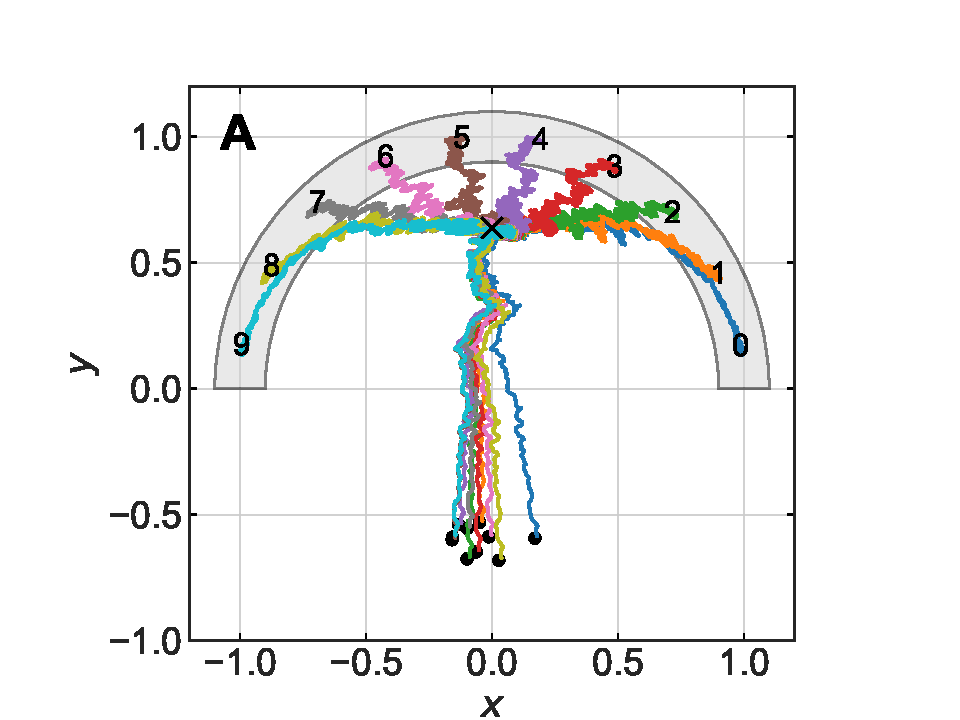
\includegraphics[width=\textwidth]{Figuras/sc_pesos_sigma_0.1_epochs_100000_lr_0.01.pdf}
            \end{subfigure}
         \begin{subfigure}[b]{\linewidth}
            \centering
            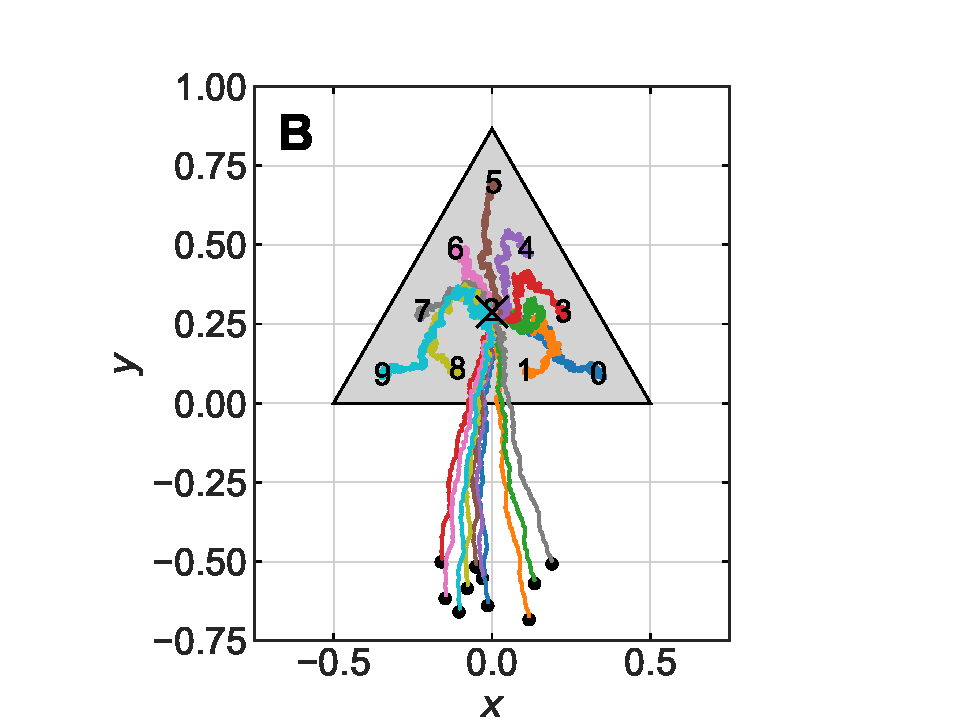
\includegraphics[width=\textwidth]{Figuras/tri_pesos_sigma_0.1_epochs_100000_lr_0.01.pdf}
         \end{subfigure}
         \begin{subfigure}[b]{\linewidth}
            \centering
            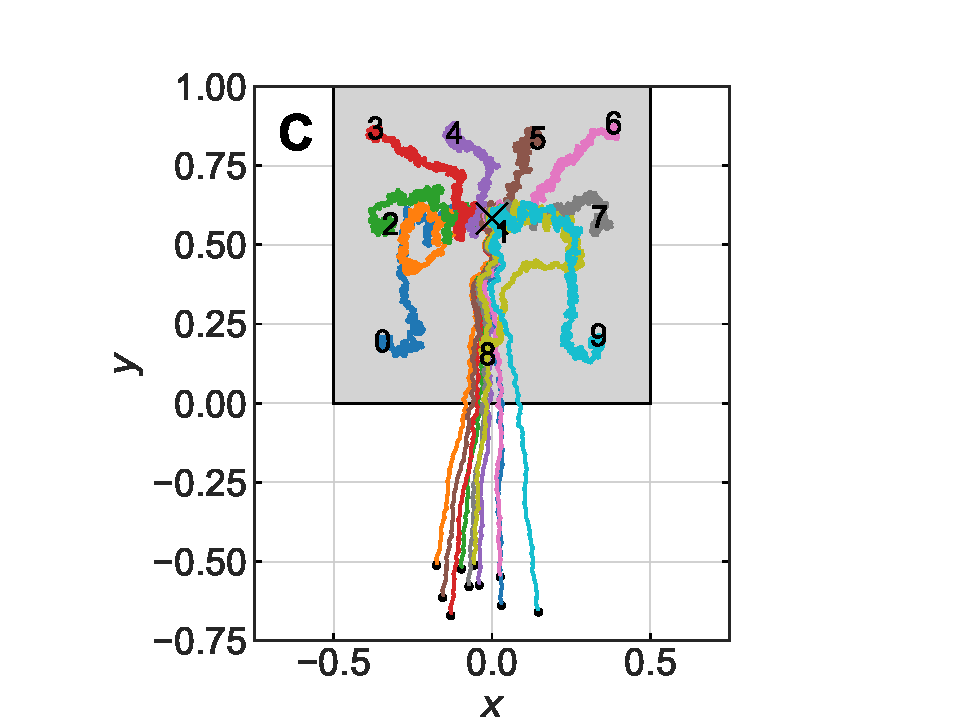
\includegraphics[width=\textwidth]{Figuras/cuad_pesos_sigma_0.1_epochs_100000_lr_0.01.pdf}
         \end{subfigure}
    \caption{Trayectoria de las neuronas de salida para una red de Kohonen con $\eta=0.01$ para $100000$ épocas para distintas topologías de la distribución de probabilidad uniforme de las neuronas de entrada (A) corona semicircular, (B) triángulo equilátero, (C) cuadrado con el doble de probabilidad de tener una entrada en la mitad superior que en la mitad inferior. Todas las neuronas empiezan distribuidas aleatoriamente y cerca entre sí. Se marca con $\times$ el centro de masa de la distribución de entradas.} 
    \label{fig:Kohonen_sigma_adp}
\end{figure}

\begin{figure}[h]
    \centering
        \begin{subfigure}[b]{\linewidth}
            \centering
            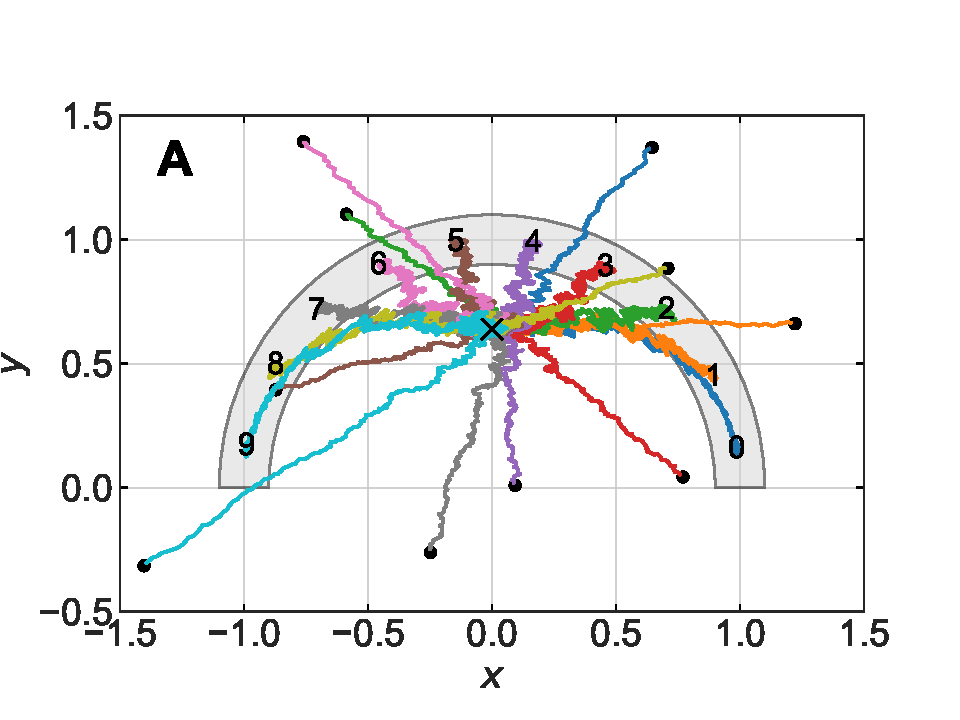
\includegraphics[width=\textwidth]{Figuras/sc_pesos_sigma_0.1_epochs_100000_lr_0.01_disp.pdf}
            \end{subfigure}
         \begin{subfigure}[b]{\linewidth}
            \centering
            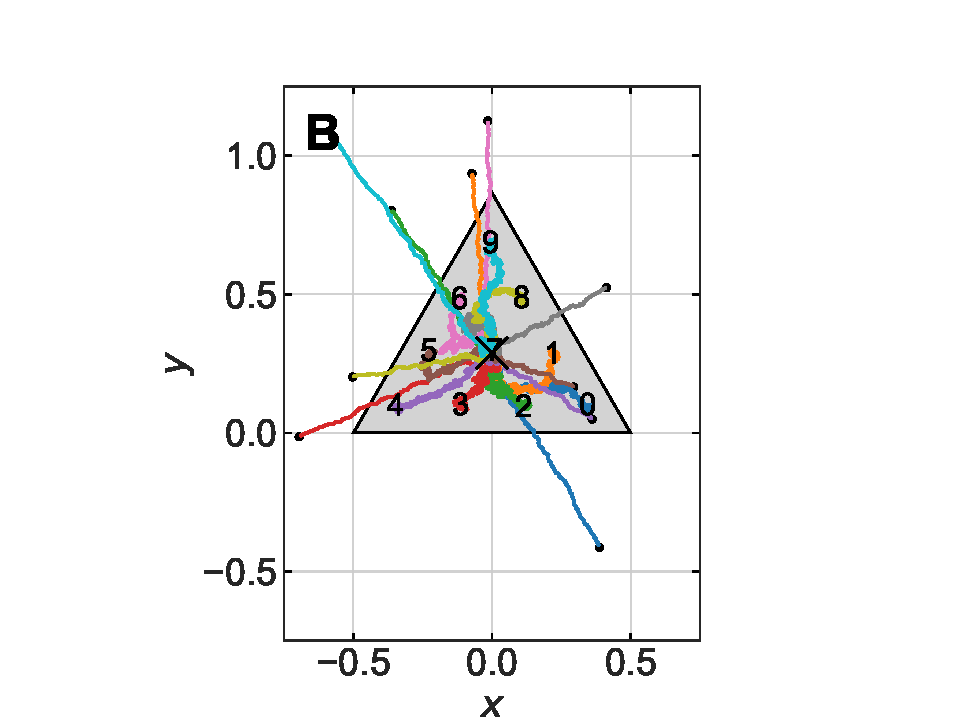
\includegraphics[width=\textwidth]{Figuras/tri_pesos_sigma_0.1_epochs_100000_lr_0.01_disp.pdf}
         \end{subfigure}
         \begin{subfigure}[b]{\linewidth}
            \centering
            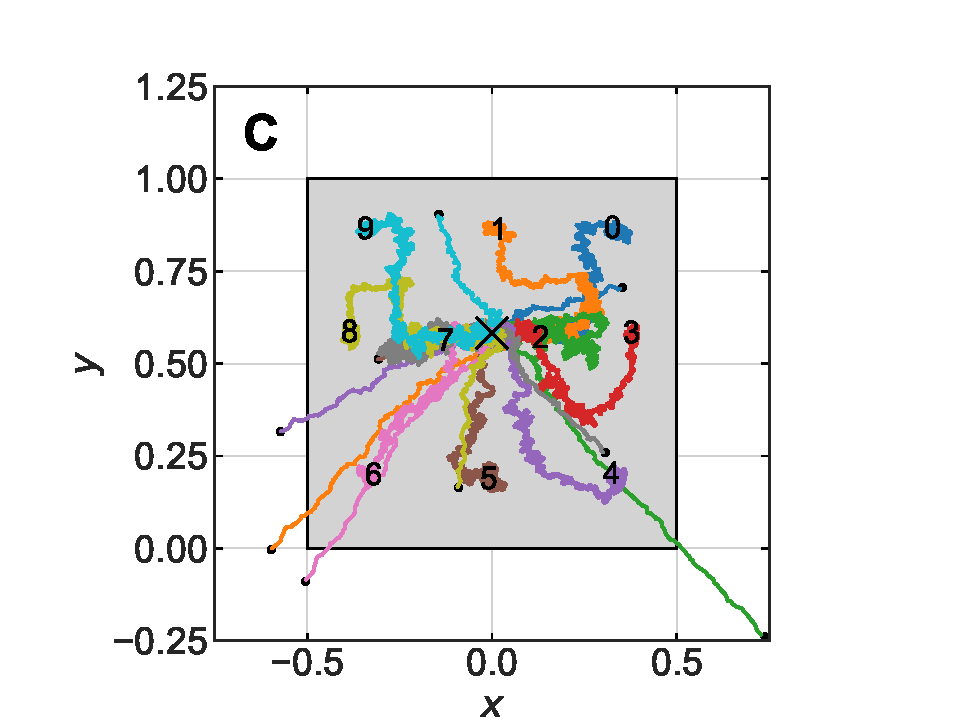
\includegraphics[width=\textwidth]{Figuras/cuad_pesos_sigma_0.1_epochs_100000_lr_0.01_disp.pdf}
         \end{subfigure}
    \caption{Trayectoria de las neuronas de salida para una red de Kohonen con $\eta=0.01$ para $100000$ épocas para distintas topologías de la distribución de probabilidad uniforme de las neuronas de entrada (A) corona semicircular, (B) triángulo equilátero, (C) cuadrado con el doble de probabilidad de tener una entrada en la mitad superior que en la mitad inferior. Todas las neuronas empiezan en distribuidas aleatoriamente en las cercanías de la topología de entrada. Se marca con $\times$ el centro de masa de la distribución de entradas.} 
    \label{fig:Kohonen_sigma_adp_dist}
\end{figure}











% Bibliography
%\renewcommand*{\bibfont}{\normalsize}
%\bibliography{Redes}

% Full bibliography added automatically for Optics Letters submissions; the following line will simply be ignored if submitting to other journals.
% Note that this extra page will not count against page length
%\bibliographyfullrefs{Redes}




\clearpage

\begin{onecolumn} % Activa una sola columna para el apéndice
\appendix
\section{Apéndice \label{codigo}}

\scriptsize
\subsection{Ejercicio 1}

\begin{lstlisting}[style=mystyle]
    import numpy as np
    import matplotlib.pyplot as plt
    from tqdm import tqdm
    
    #Ploteo 
    import seaborn as sns
    #sns.axes_style("whitegrid")
    sns.set_style("ticks")
    
    
    Sigma = np.array([
        [2,1,1,1],
        [1,2,1,1],
        [1,1,2,1],
        [1,1,1,2]
    ])
    
    sqrtSigma = np.array([
        [1.309, 0.309, 0.309, 0.309],
        [0.309, 1.309, 0.309, 0.309],
        [0.309, 0.309, 1.309, 0.309],
        [0.309, 0.309, 0.309, 1.309]
    ])
    
    #Arquitectura de la red
    input_size = 4
    output_size = 1
    learning_rate = 0.01
    num_epochs = 250
    fig_index = "A"
    epochs = [i for i in range(0, num_epochs)]
    
    w_plot = np.zeros((num_epochs, input_size))
    dot_plot = np.zeros((num_epochs, input_size))
    
    # Pesos iniciales aleatorios
    w = np.random.uniform(-0.1,0.1,size=(output_size, input_size)) #filas #columnas
    
    autovalores, autovectores = np.linalg.eig(Sigma)
    
    print("Autovalores de Sigma:")
    print(autovalores)
    print("Autovectores de Sigma:")
    print((autovectores.T[1]).reshape(-1, 1))
    print("\n")
    
    for epoch in tqdm(range(num_epochs)):
    
        w_plot[epoch] = w
        z_train = np.random.multivariate_normal([0,0,0,0], Sigma)
        x_train = np.dot(sqrtSigma,z_train)
    
        O = np.dot(w, x_train)
    
        for i in range(input_size):
            dot_plot[epoch][i] = np.dot(w, autovectores.T[i].reshape(-1, 1))
        
        # Actualizacion de pesos
        w += learning_rate*O*(x_train-O*w)
    
    print("Entrenamiento completado.")
    
    fig1, ax1 = plt.subplots(figsize=(8,6))
    for i in range(input_size):
        ax1.plot(epochs, w_plot[:,i], "-", label = r"$w_{" + str(i) + "}$")
    ax1.hlines(y=0.5,  xmin=0, xmax=num_epochs, linestyle='--', color='gray')
    ax1.hlines(y=-0.5,  xmin=0, xmax=num_epochs, linestyle='--', color='gray')
    ax1.set_xlabel(r"Epoca", fontsize=18)
    ax1.set_ylabel(r"Pesos $w_j$", fontsize=18)
    ax1.tick_params(direction='in', top=True, right=True, left=True, bottom=True)
    ax1.tick_params(axis='x', rotation=0, labelsize=18, color='black')
    ax1.tick_params(axis='y', labelsize=18, color='black')
    ax1.legend(fontsize=12, framealpha=1, loc= "center right")
    ax1.set_xlim(0, num_epochs)
    ax1.text(0.05, 0.9, f'{fig_index}' , transform=ax1.transAxes, fontsize=24, verticalalignment='top', fontweight='bold', color="black")
    ax1.grid(True, linewidth=0.5, linestyle='-', alpha=0.9)
    fig1.savefig(f"../Redes-Neuronales/Practica_5/resultados/ej1/pesos_lr_{learning_rate}.pdf")
    fig1.savefig(f"../Redes-Neuronales/Practica_5/resultados/ej1/pesos_lr_{learning_rate}.png", dpi=600)
    
    fig2, ax2 = plt.subplots(figsize=(8,6))
    for i in range(input_size):
        ax2.plot(epochs, dot_plot[:, i], "-", label=r"$\vec{w} \cdot \vec{v_" + str(i) + "}$")
    ax2.hlines(y=1.0,  xmin=0, xmax=num_epochs, linestyle='--', color='gray')
    ax2.hlines(y=-1.0,  xmin=0, xmax=num_epochs, linestyle='--', color='gray')
    ax2.hlines(y=0.0,  xmin=0, xmax=num_epochs, linestyle='--', color='gray')
    ax2.set_xlabel(r"Epoca", fontsize=18)
    ax2.set_ylabel(r"Producto escalar $\vec{w} \cdot \vec{v_j}$", fontsize=18)
    ax2.tick_params(direction='in', top=True, right=True, left=True, bottom=True)
    ax2.tick_params(axis='x', rotation=0, labelsize=18, color='black')
    ax2.tick_params(axis='y', labelsize=18, color='black')
    ax2.legend(fontsize=12, framealpha=1, loc= "upper right")
    ax2.set_xlim(0, num_epochs)
    ax2.text(0.05, 0.9, f'{fig_index}', transform=ax2.transAxes, fontsize=24, verticalalignment='top', fontweight='bold', color="black")
    ax2.grid(True, linewidth=0.5, linestyle='-', alpha=0.9)
    fig2.savefig(f"../Redes-Neuronales/Practica_5/resultados/ej1/prodesc_lr_{learning_rate}.pdf")
    fig2.savefig(f"../Redes-Neuronales/Practica_5/resultados/ej1/prodesc_lr_{learning_rate}.png", dpi=600)


\end{lstlisting}
\subsection{Ejercicio 2}
\begin{lstlisting}[style=mystyle]
import numpy as np
import matplotlib.pyplot as plt
from tqdm import tqdm
#Ploteo 
import seaborn as sns
import matplotlib.patches as patches
#sns.axes_style("whitegrid")
sns.set_style("ticks")

def gaussian(i, i_, sigma):
    return np.exp(-(((i-i_)**2)/(2*(sigma**2))))

def input_semicircle():
    f = True
    while f:
        x = np.random.uniform(-1.1,1.1)
        y = np.random.uniform(0,1.1)

        r = np.linalg.norm([x,y])
        if( 0.9 <= r <= 1.1 and 0 <= np.arctan2(y,x) <= np.pi ):
            f = False
    return np.array([x,y])

def input_triangle():
    f = True
    while f:
        x = np.random.uniform(-0.5,0.5)
        y = np.random.uniform(0.0,np.sqrt(3)/2)
                
        if ( -0.5 <= x <= 0.5 and 0 <= y <= np.tan(np.pi/3)*(0.5-np.abs(x)) ):
            f = False
    #ax1.plot(x, y, marker='o', markersize=1, color='k')     
    return np.array([x,y])

def input_square():
    f = True
    while f:
        x = np.random.uniform(-0.5,0.5)
        y = np.random.uniform(0.0,2.0)
        # Verifica si el punto esta en la mitad inferior del cuadrado
        if (-0.5 <= x <= 0.5) and (0.0 <= y <= 1.0):
            # Genera un numero aleatorio adicional para duplicar la probabilidad en la mitad inferior
            if y <= 0.5:
                if np.random.rand() <= 0.5:
                    f = False
            else:
                f = False
    #ax1.plot(x, y, marker='o', markersize=0.5, color='k')  
    return np.array([x,y])

#Arquitectura de la red
input_size = 2
output_size = 10
learning_rate = 0.01
sigma_0 = 10000
#sigma = 1.0
num_epochs = 100000
fig_index = "C"
epochs = [i for i in range(0, num_epochs)]

w_plot = np.zeros((num_epochs, input_size))

w = np.array([[np.random.uniform(-0.75, 0.75), np.random.uniform(-0.25, 1.25)] for _ in range(output_size)])

"""
w = np.array([[ 0.1389785 ,  0.02162108],
 [ 0.00636808 ,  0.16040874],
 [ 0.05046116 , 0.0006476 ],
 [ 0.15113858 , 0.04233544],
 [ 0.08499907 , 0.13616288],
 [-0.09924555 , 0.15332305],
 [-0.00520648 ,  0.08107896],
 [-0.18375063 , 0.15545262],
 [-0.03089037 , 0.15672824],
 [-0.06498289 ,  0.07104595]])
"""

plot_w = np.zeros((num_epochs, output_size, input_size))

fig1, ax1 = plt.subplots()

for i in range (output_size):
    ax1.plot(w[i, 0], w[i, 1], 'o',  color='k', markersize = 3)

for epoch in tqdm(range(num_epochs)):
    x = input_square()
    norm = np.linalg.norm(w - x, axis=1)
    i_ = np.argmin(norm)
    sigma = sigma_0/(epoch+1)
    # Actualizacion de pesos
    for i in range(output_size):
        w[i] += learning_rate*gaussian(i,i_,sigma)*(x-w[i])
        plot_w[epoch][i] = w[i]

for i in range ( output_size ):
    ax1.text(w[i, 0], w[i, 1], str(i), fontsize=15, ha='center', va='center', color='k')


for i in range(output_size):
    x_trajectory = plot_w[:, i, 0]
    y_trajectory = plot_w[:, i, 1]
    plt.plot(x_trajectory, y_trajectory, label=f"Neurona {i+1}")

print("Entrenamiento completado.")

ax1.set_xlabel(r"$x$", fontsize=18)
ax1.set_ylabel(r"$y$", fontsize=18)
ax1.tick_params(direction='in', top=True, right=True, left=True, bottom=True)
ax1.tick_params(axis='x', rotation=0, labelsize=18, color='black')
ax1.tick_params(axis='y', labelsize=18, color='black')
#ax1.legend(fontsize=12, framealpha=1)
#ax1.set_xlim(-1.2, 1.2)
#ax1.set_ylim(-0.1, 1.2)
ax1.text(0.05, 0.95, f'{fig_index}' , transform=ax1.transAxes, fontsize=24, verticalalignment='top', fontweight='bold', color="black")
ax1.grid(True, linewidth=0.5, linestyle='-', alpha=0.9)
ax1.set_aspect('equal')

#ax1.plot(0, 0.6387, marker='x', markersize=10, color='k', label='Centro de masa')
ring = patches.Wedge(center=(0, 0), r=1.1, theta1=0, theta2=180, width=0.2, facecolor='lightgray', edgecolor='black', alpha=0.5)
ax1.add_patch(ring)
ax1.set_xlim(-1.5, 1.5)
ax1.set_ylim(-0.5, 1.5)

#triangle = patches.Polygon(np.array([[-0.5, 0], [0.5, 0], [0, np.sqrt(3) / 2]]), closed=True, facecolor='lightgray', edgecolor='black')
#ax1.add_patch(triangle)
#ax1.plot(0, 0.28867, marker='x', markersize=15, color='k', label='Centro de masa')
#ax1.set_xlim(-0.75, 0.75)
#ax1.set_ylim(-0.75, 1.25)

#square = patches.Rectangle((-0.5, 0), 1, 1, angle=0, facecolor='lightgray', edgecolor='black')
#ax1.add_patch(square)
#ax1.plot(0, 0.583, marker='x', markersize=15, color='k', label='Centro de masa')
#ax1.set_xlim(-0.75, 0.75)
#ax1.set_ylim(-0.25, 1.25)

fig1.savefig(f"../Redes-Neuronales/Practica_5/resultados/ej2/pesos_sigma_{sigma}_epochs_{num_epochs}_lr_{learning_rate}.pdf")
fig1.savefig(f"../Redes-Neuronales/Practica_5/resultados/ej2/pesos_sigma_{sigma}_epochs_{num_epochs}_lr_{learning_rate}.png", dpi=600)

\end{lstlisting}

\end{onecolumn}

\end{document}


